\documentclass{article}
\usepackage{acra}
\usepackage{graphicx}
\usepackage{url}
\title{A Four-Arm Assembly Line for a Three-Part Fidget Toy}
\author{Group 4 \\ ENGMT558 Robotics \\ University of Waikato}
% Replace each value after the physical lab trials; do not enter simulated results here.
\newcommand{\PhysicalTrials}{\textit{not measured}}
\newcommand{\PhysicalSuccesses}{\textit{not measured}}
\newcommand{\MeanCycleTime}{\textit{not measured}}
\newcommand{\MaxPositionError}{\textit{not measured}}
\newcommand{\GoodAccepted}{\textit{not measured}}
\newcommand{\MissingGearResult}{\textit{not measured}}
\newcommand{\InsertResult}{\textit{not measured}}
\newcommand{\EmergencyStopResult}{\textit{not measured}}
\newcommand{\CameraBypasses}{\textit{not measured}}

\begin{document}
\maketitle
\begin{abstract}
This project develops a ROS 2 assembly line using four SO101 manipulators, a conveyor, an ESP32 interface and camera inspection. Two arms assemble a three-part fidget toy while two downstream arms prepare its packaging. The design separates motion, inspection and low-level I/O, allowing the same process requirements to be tested with a desktop micro-ROS client before connecting the physical control board. The simulation uses the supplied rig and product CAD, measured joint feedback and explicit attachment checks. This report describes the implementation and the evidence available during development. Physical grip calibration, defect-classification accuracy and the five assessed production trials remain to be measured; simulated attachments are not evidence of a successful physical snap-fit.
\end{abstract}

\section{Requirements and system design}
The project brief requires assembly, inspection and packaging on a fixed conveyor rig \cite{brief}. A successful cell must perform at least three assembly operations, detect two different product defects, remove rejected products and package accepted products. Start, pause, emergency stop, mode selection, tower lights, alarm and the conveyor proximity sensor form part of the assessed integration \cite{rubric}.

The cell is divided into three cooperating jobs: assembly, conveyor transfer and packaging. Assembly uses arms 1 and 2. Arm 3 inspects the completed toy and places it into the box. Arm 4 prepares the empty box, handles the lid and transfers the finished package. This allocation lets the packaging station prepare while construction is underway, without requiring all four arms to enter one shared workspace.

The coordinator runs on the ROS 2 computer. The micro-ROS agent connects it to an ESP32 for physical I/O or to a desktop micro-ROS client for simulation. A separate camera node receives inspection requests and publishes a result associated with that request. Network addresses, camera source and provisional GPIO assignments are collected in \texttt{ID.yaml}. Station poses and captured joint overrides are separate from network settings so calibration does not require editing the sequence code.

\subsection{Equipment and communication}
The supplied system diagram includes a robot-driver computer, follower and leader arms, a planning computer, an Ethernet router, and either a USB camera or a Wi-Fi camera server \cite{diagram}. The camera is mounted on the conveyor inspection arm; a laptop camera is not assumed. The implementation supports a USB video device, a configured stream URL or a ROS image topic. The actual device or endpoint must be selected on the lab computer.

The university driver launch commands are identified in the diagram, but the supplied resources do not include their ROS message definitions or joint-unit conversion. Consequently, the physical display accepts configured \texttt{JointState} feedback and remains read-only. A complete physical motion connection requires confirmation of the lab command topics, names, offsets, limits and gripper units. Gazebo trajectory topics must not be assumed to match that interface.

\subsection{Emergency stop and signal levels}
The physical emergency stop must remove the actuator or relay supply independently of ROS and firmware. An isolated feedback input can report its state to the coordinator, but software is not the power-cut mechanism. The ESP32 uses 3.3V logic. Relay supplies and any higher-voltage sensor output require a suitable interface. GPIO35 is input-only and has no internal pull-up or pull-down; its input bias is external \cite{esp}.

The connector sketch assigns Start to GPIO4, Pause to GPIO2, selector to GPIO16, proximity to GPIO35, and step/direction/enable to GPIO18/19/21. Tower green/yellow/red/alarm are GPIO26/25/33/32. Input polarity, connector orientation, emergency-stop feedback and driver timing remain commissioning items. Firmware output enable stays locked until these have been checked.

\begin{figure*}[t]
\centering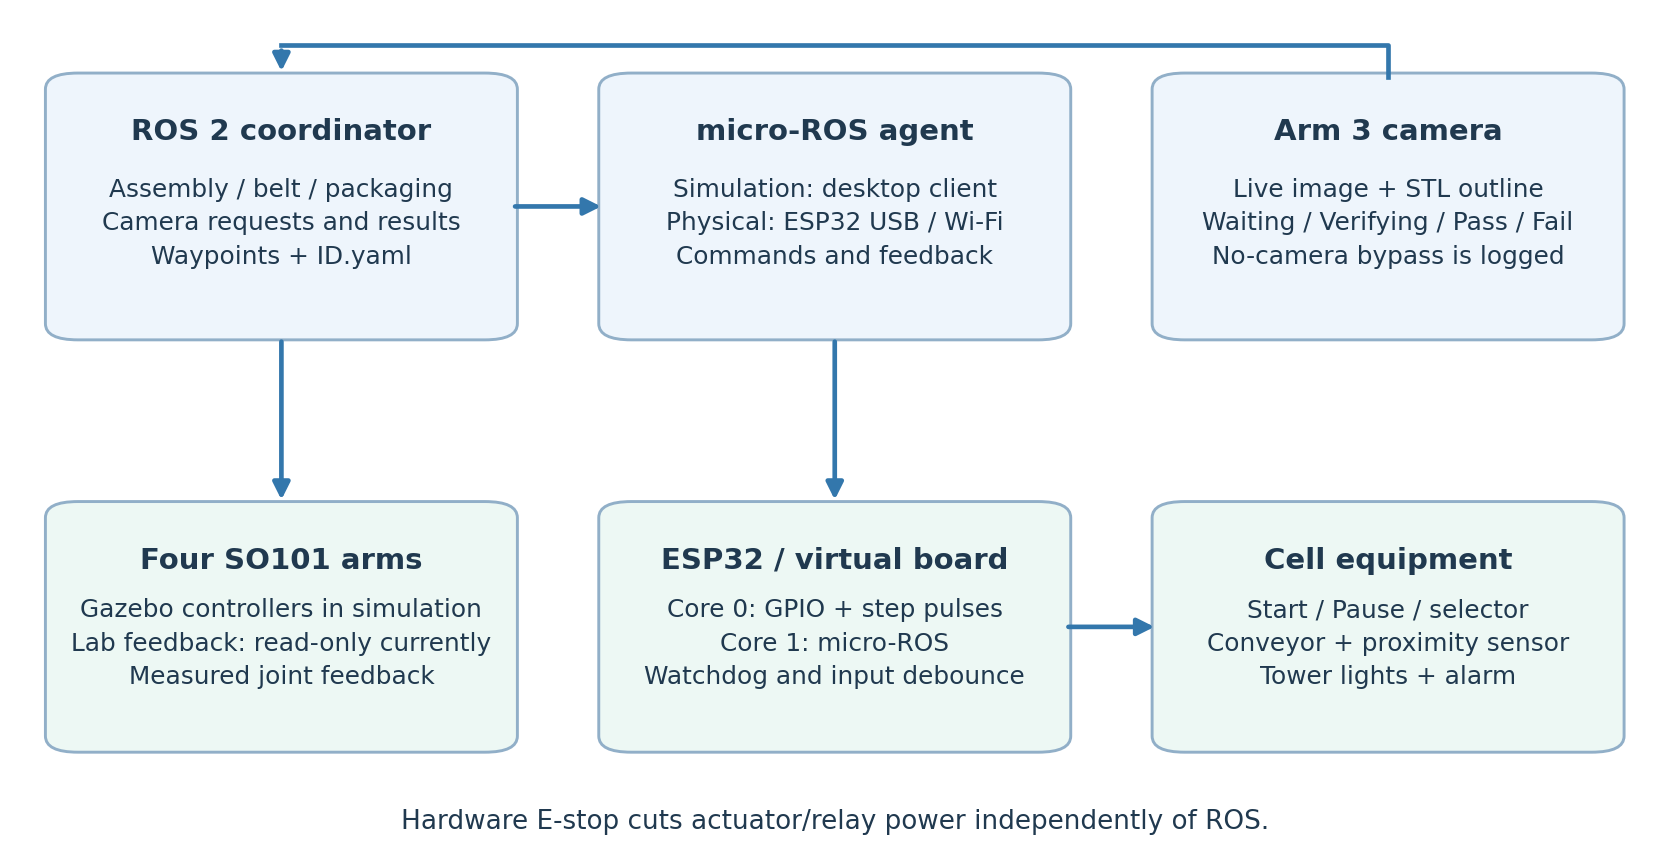
\includegraphics[width=\textwidth]{architecture.png}
\caption{Control and communication architecture. Simulation and physical I/O use separate configurations. The emergency power cut is independent of software.}
\label{fig:architecture}
\end{figure*}

\section{Product and process}
The final product has a base, a gear and an end insert. The supplied V6 base is approximately $76.89\times28\times18$mm; the gear diameter is approximately 28.2mm. The base remains rod-up. The gear fits onto the upper rod, and the insert enters through an end. The intended manipulation tasks are oriented pickup and placement, end insertion and a final pinch to seat the retaining features. CAD establishes nominal mating positions; it does not establish printed tolerances, insertion force or grip reliability.

\subsection{Final feeder and fixture arrangement}
The hardware uses five removable carrier plates, each holding an insert, gear and base, left to right when viewed from the assembly side. They fill the inclined rack. The V6 exports include the parts, carrier and separate bench assembly jig. The runtime part meshes and camera reference now use V6, retaining the measured mating datums from V5. Dimension, seated-level and camera-reference tests pass. The connected carrier and fixed assembly jig are loaded. The loaded carrier uses its centre front tab; its pickup still stalls in the live collision model. Offline contact checks alone have not resolved that live obstruction.

The requested assembly jig uses existing bench holes, with three locating pins in each of two adjacent rows. The final pose needs measurement. The intended sequence draws a loaded carrier down by its centre front tab, transfers parts into the assembly jig and discards the empty carrier to the left after assembly. No extra bench rails are required. The simulated rig sits on a 1m table. Feeder advancement is prescribed motion, not a validated model of friction or gravity feeding.

\subsection{Construction and transfer}
Arm 1 collects the gear while arm 2 prepares the base. Shared-space placement is serialised. Arm 1 fits the gear and stages the end insert; arm 2 inserts it, releases, repositions above the product and pinches the insert and body together. The finished toy should then move to the conveyor without a new grasp. This is the final requested sequence. The current sequence still uses a separate finished-toy pickup, so the pinch-and-carry action requires replacement waypoints.

The conveyor has an input position, an inspection/output position and a transfer state. Loading requires a stopped belt and clear input. Transfer requires a clear output. Arrival must stop the belt; pickup must clear the sensor before the next transfer. A downward range beam provides simulated object detection through the micro-ROS client. The real proximity signal requires polarity and position calibration. The input/output interlocks allow assembly to continue while a prior toy is inspected, without advancing another toy into an occupied output.

\subsection{Inspection and packaging}
Arm 4 prepares an empty box while assembly proceeds. Arm 3 positions its camera to view the toy on the stopped conveyor. Accepted toys are placed long-axis to long-axis inside the box. Arm 3 withdraws before arm 4 fits the lid, grips the box body sides and places the package on the output tray. The fixed order is the far pair, near pair, then a fifth box centred above them. A rejected toy goes to a separate bench location; the prepared box is retained for the next accepted product.

The camera node supports a USB device, network stream or ROS image topic. It displays Waiting while idle and Verifying only for an active inspection request. Closing the camera releases its stream; the panel can reopen it. The GTK visibility fallback was corrected and an open/close/open/close GUI test passed with the CAD camera source. Operator closure produces an inspection failure rather than a no-camera pass. It compares contours with projections of the assembled CAD. The required defects are a missing gear and an incompletely seated insert. The top silhouette alone can hide the insert fault, so a second angled view is included. Viewpoint, lighting, background and the camera-to-tool transform need lab calibration. A missing-camera bypass is explicitly recorded and cannot count as a correct inspection decision.

\section{Software implementation}
ROS 2 Humble coordinates four Gazebo trajectory controllers. Each move waits for fresh joint feedback within 0.003rad and a tool-position error below 0.5mm. The modeled contact target is 1mm; this is not a claim of physical accuracy. Waiting arms are monitored for drift. Small corrections are collision-checked; excessive drift or stale feedback stops the sequence. Encoders cannot measure structural flex, backlash or a slipped product.

A sampled swept-volume check compares a proposed arm movement with the other arms. Assembly and packaging may overlap, but operations sharing a station are ordered. This interlock is not a proof of continuous collision freedom: fixture clearances, held objects and actual joint calibration still need separate checks.

\subsection{Grasp model and current limitation}
Gazebo fixed attachments represent grasping and completed insertions. Both finger pads must be within 1mm of the STL surfaces before attachment. The gear check uses opposite outer contacts, excluding the centre bore. Placement checks alignment before attaching components. This prevents the previous tool-centre test from accepting an apparent grasp with the fingers in free space.

The box body and lid are separate meshes. Product vertices are checked against the box cavity, and closed-box pickup is checked against the lid. The latest side-grip plan fails its contact, placement or lid-clearance check; the affected stack action therefore waits. Full-task Start now runs the available paths, and independent stations continue when a movement is blocked. The tolerance has not been widened to conceal the problem. The simulation does not model snap-fit deformation or prove frictional grip strength. A successful attachment is not evidence of physical insertion force or retention.

\subsection{Controls and path editing}
The ESP32 uses separate tasks for hardware handling and micro-ROS. The hardware task debounces inputs, controls lights and generates conveyor pulses. A stale command heartbeat stops pulses and removes restart permission. A disabled command with healthy feedback must precede re-enabling motion. A desktop micro-ROS client implements the equivalent simulated inputs and loads; its agent starts with the simulator.

The panel provides Full task, Assembly, Inspection and Packaging selections, product count and Reset. Fault count and placement are selectable, and product outcome squares are separate from board outputs. The current standalone-stage loading behaviour still needs the final requested short conveyor advancement and one-at-a-time holder updates. The physical control merge and mode-selector reset behaviour also require completion and commissioning.

Plan a path opens a separate window with four ordered arm columns. Clicking a task shows its named movements and live joint readings. Measured positions can be saved, overwritten or removed; tasks and movements can be reordered for teaching replay. Each replay move uses feedback and other-arm clearance checks. Solved reference coordinates are saved with a geometry signature; changing station geometry invalidates them. Unsolved paths remain explicitly listed rather than receiving placeholder joint values. Overwriting a named production target updates its joint override. New teaching tasks do not silently replace automatic assembly dependencies. That sequence remains editable separately, so path timing cannot accidentally remove a station interlock.

\section{Validation and remaining measurements}
Development checks distinguish protocol tests, geometric checks, simulated production and physical trials. The current automated suite passes 106 tests. A live Full diagnostic run with five products accepted Start, Pause and resume. When the carrier pickup stalled, assembly held its measured joints while packaging continued. The controller remained RUNNING and reported the blocked station. A separate earlier test restored the scene and replayed a manual movement. These results do not establish a complete production cycle.

The main ESP32 was compiled and flashed successfully over USB, and the micro-ROS agent received its fourteen-field telemetry message. Actuator output verification remained disabled. This verifies the communication path only: physical button transitions, sensor polarity, conveyor timing and the independent emergency power cut were not demonstrated in that test.

The laptop panel offers Wi-Fi/laptop ROS and USB/lab-PC ROS connection profiles. A separate observer process reads the hardware domain while the simulator stays isolated. The supplied lab-PC agent scripts leave the university arm-driver workspace intact. Motor commands remain disabled until the driver message types, joint order, units and limits are checked. An ESP32 connection alone does not prove that the four arms can be commanded.

An earlier V5 baseline recorded a complete simulated cycle and a separate four-good/two-defect QA trial. Those historical results are not attributed to the revised V6 setup. The current revision has ten solved task references (40 joint movements). Five closed-box stacking paths are still unresolved. A diagnostic run is not a completed batch; the V6 five-product run has not passed. Final geometry, single-stage stock handling and physical-control integration must be retested after the remaining changes.

\begin{table}[h]
\centering\small
\begin{tabular}{p{0.43\columnwidth}p{0.46\columnwidth}}
\hline
Check & Current evidence/status \\
\hline
Automated software tests & 106 passed \\
Reset and teaching & Live simulation checks passed \\
ESP32 USB telemetry & Received; outputs disabled \\
Closed-box pickup & Clearance/placement failure \\
V6 parts / carrier workflow & Loaded; pickup clearance pending \\
Physical snap-fit and grip & Not measured \\
Camera: 4 good, 2 flawed & Lab trial required \\
Five consecutive cycles & Revised full trial required \\
Physical cycle time & Not measured \\
\hline
\end{tabular}
\caption{Current revision evidence. Historical baseline runs do not validate changed geometry or trajectories.}
\end{table}

\subsection{Acceptance trial}
Before an assessed run, record all four arms' feedback and command conventions, capture low-speed approach and contact waypoints, and verify that the base rod remains uppermost. Check each pickup, insertion, release and withdrawal individually. Verify that parts and boxes sit on their real support surfaces and that subsequent feeder items advance without bridging or double-feeding.

For inspection, randomise four correctly assembled toys and one sample of each specified defect. Record the predicted label, actual condition, image and rejection action. A no-camera bypass must be recorded separately. Report the two defect detection results individually; an overall acceptance rate can hide failure to detect one defect class.

Run five production trials with timestamps for Start, assembly completion, conveyor transfer, inspection and packed output. Count consecutive complete successes, not merely successful robot moves. Report total cycle time and the time spent waiting at each station. These measurements establish whether overlapping preparation reduces idle time and whether the conveyor interlocks prevent conflicts when the two stations run at different rates.

\subsection{Physical results to complete}
Record the measured data in the supplied CSV sheets and enter the summary values
in \texttt{results.tex}. Physical complete cycles: \PhysicalSuccesses{} of
\PhysicalTrials{}. Mean complete-cycle time: \MeanCycleTime{}.
Maximum measured pickup/placement error: \MaxPositionError{}.
Correct good-part decisions: \GoodAccepted{} of four;
missing-gear rejection: \MissingGearResult{};
unseated-insert rejection: \InsertResult{}.
Emergency power-cut check: \EmergencyStopResult{}.
Report camera bypasses separately: \CameraBypasses{}.

\section{Conclusion}
The implementation provides a configurable coordinator, micro-ROS protocol testing, camera inspection scaffolding and CAD-based simulation. USB telemetry and isolated teaching tests have been demonstrated. The final V6 scene and closed-box transfer still need correction and a new complete-cycle test. Claims of reliable physical assembly, real-camera defect detection and throughput require the measured trials described above.

\small
\begin{thebibliography}{9}
\bibitem{brief} ENGMT558. Project 2: Autonomous Assembly Line. Supplied project handout, 2026.
\bibitem{rubric} ENGMT558. Project 2 Autonomous Assembly Line: Assessment Rubric. Supplied rubric, 2026.
\bibitem{diagram} ENGMT558. System Block Diagram, version 2. Supplied rig architecture, 2026.
\bibitem{esp} Espressif Systems. ESP32 GPIO and RTC GPIO. \url{https://docs.espressif.com/projects/esp-idf/en/stable/esp32/api-reference/peripherals/gpio.html}.
\end{thebibliography}
\end{document}
